\documentclass[a4paper,12pt]{report}
\usepackage[T1]{fontenc}
\usepackage[utf8]{inputenc}
\def\magyarOptions{defaults=hu-min}
\usepackage[magyar]{babel}
\usepackage{amsthm, amssymb,amsmath,hyperref}
\usepackage{enumerate, graphicx, xcolor}
\usepackage{caption,setspace}

\usepackage{pdfpages}

\usepackage{chngcntr}
\counterwithout{figure}{chapter}
\counterwithout{figure}{section}
\counterwithout{figure}{subsection}

\counterwithin{figure}{chapter}
%\usepackage{pgf,tikz,float}
%\usepackage{tikzlings}
%\usepackage{tikzducks}
%\usetikzlibrary{arrows}
%\usepackage[nobysame]{amsrefs}
%\usepackage{amsmath}

\usepackage{geometry}
 \geometry{
 a4paper,
 total={160mm,247mm},
 left=25mm,
 top=25mm,
 }


\newtheorem{theo}{tétel}[section]
\newtheorem{defin}[theo]{definíció}
\newtheorem{lemma}[theo]{lemma}
\newtheorem{all}[theo]{állítás}
\newtheorem{kov}[theo]{következmény}

\theoremstyle{definition}
\newtheorem{definition}[theo]{definíció}

\theoremstyle{remark}
\newtheorem{megj}[theo]{megjegyzés}




\date{today}

\linespread{1.3}

\usepackage{listings}
\usepackage{color}

\definecolor{dkgreen}{rgb}{0,0.6,0}
\definecolor{gray}{rgb}{0.5,0.5,0.5}
\definecolor{mauve}{rgb}{0.58,0,0.82}

\lstset{frame=tb,
  language=Java,
  aboveskip=3mm,
  belowskip=3mm,
  showstringspaces=false,
  columns=flexible,
  basicstyle={\small\ttfamily},
  numbers=none,
  numberstyle=\tiny\color{gray},
  keywordstyle=\color{blue},
  commentstyle=\color{dkgreen},
  stringstyle=\color{mauve},
  breaklines=true,
  breakatwhitespace=true,
  tabsize=3
}



\begin{document}


\pagenumbering{roman}

%Elso  oldal 
\thispagestyle{empty}

\begin{center}
\vspace*{0.2cm} {\Large\bf Szegedi Tudományegyetem}
\vspace{0.3cm}

{\Large\bf Természettudományi és Informatikai Kar}
\vspace{0.3cm}

{\Large\bf Informatikai Intézet, Szoftverfejlesztés Tanszék}
\vspace{3cm}



{\Large SZAKDOLGOZAT}

\vspace*{1.5cm}

{\LARGE\bf Eseményszervező webalkalmazás konfigurációs lehetőségekkel}

Configurable event organizing web application



\vspace*{4cm}

{\large
\begin{tabular}{c@{\hspace{2cm}}c}
\emph{Készítette:}     &\emph{Témavezető:}\\
\bf{Koncz Máté}  &\bf{Dr. Pengő Edit}\\
Programterveő Informatikus BSc hallgató    & egyetemi adjunktus\\
&
\end{tabular}
}

\vspace*{1,5cm}

{\Large Szeged\\ \vspace{2mm} 2025}
\end{center}

%masodik oldal osszefogalalo

\newpage

{\Huge \bf Feladatkiírás}

\bigskip
%\setlength{\parskip}{\baselineskip}%

A cél egy eseményszervezést segítő webalkalmazás létrehozása Angular-ban, amely egy Spring keretrendszerre épülő API-t használ. A szükséges adatokat az alkalmazás egy relációs adatbázis szerveren tárolja. Az alkalmazás nagyobb baráti társaságoknak készül segítségként, hogy találkozásokhoz megtalálják a legmegfelelőbb időpontot, és mindig értesüljenek az eseményt érintő változásokról. A felhasználók eseményeket készíthetnek, ezekhez más felhasználók egy csoportját társíthatják. Ezután az esemény tulajdonosa meghirdeti a releváns információkat és a lehetséges időpontokat. Ezekre a részvevők egy naptár felületen reagálhatnak ( jó időpont, rossz időpont, elfogadható időpont). Ezekről az adatokról a szervező informatív statisztikákat kap. Az eseményekből sémák készíthetőek, amelyek segítségével új eseményeket lehet létrehozni. Az alkalmazás fontos része a résztvevők állandó tájékoztatása az esemény híreiről (pl. időpont véglegesítése, esemény lemondása, helyszín változás). Továbbá fontos az adatok biztonsága, vagyis hogy illetéktelenek (nem résztvevők) ne férhessenenek hozzá az események adataihoz.

\newpage

{\Huge \bf Tartalmi összefoglaló:}

\bigskip

{\bf Téma megnevezése}

\medskip

Eseményszervezést segítő webalkalmazás készítése, amely egy adott társaság összeszervezése mellett alkalmas eseménysémák létrehozására és azok konfigurálására is.

\bigskip

{\bf Megoldási mód}

\medskip

Létrehoztam egy Angular keretrendszerben megvalósított webalkalmazást, amely az általam Spring Boot keretrendszerben írt API-t használja REST végpontokon keresztül. Az eseményszervezéshez szükséges logikát a backend oldalon valósítottam meg, a frontend oldali webalkalmazásnak csak a felhasználóval folytatott interakciókban van szerepe.

\bigskip

{\bf Alkalmazott eszközök, módszerek}

\medskip

A fejlesztés során az InteliJ IDEA és a Visual Studio Code fejlesztőkörnyezeteket használtam. A backend felépítését a Controller-Service-Repository architektúrális tervezési minta alapján alkottam meg.	

\bigskip

{\bf Elért eredmények}

\medskip

Az alkalmazás használatával eseményeket lehet létrehozni, lehetőség van azok konfigurációjára és sokszorosítására. Az eseményekhez más felhasználók is adhatók, az általuk adott visszajelzésekről könnyen értelmezhető statisztikákat kap az esemény szervezője. Az események adatainak véglegesítéséről a felhasználók alkalmazáson belüli üzenetben értesülnek.

\bigskip

{\bf Kulcsszavak}

\medskip

alkalmazás, eseményszervezés, frontend, backend, Angular, Spring Boot


\newpage

\pagebreak

\tableofcontents
\pagebreak
%\listoffigures
%\pagebreak


\chapter{Bevezetés}
\pagenumbering{arabic}

\section{Motiváció}

Az alkalmazás ötlete még gimnazista koromban született meg. Az osztálytársaimmal gyakran jártunk össze focizni, ám ezeket az alkalmakat mindig komoly kihívás volt megszervezni. Az legtöbb alkalom azért maradt el, mert nem sikerült olyan időpontot találni, amelyre legalább 8 ember biztosan el tudott jönni. A szavazások nehezen folytak le, rendszerint a messenger-en küldött 'foci péntek délután?', 'foci szombat délelőtt?' stb. üzenetekre adott reakciók száma alapján dőlt el a focizás időpontja. Az alkalmazásom az ehhez hasonló események szervezését könnyíti meg, ahol a legnagyobb kihívás az ideális időpont megtalálása, hiszen az a legfontosabb, hogy az minél több embernek feleljen meg. A focizáshoz az időponton kívül a helyszínt is el kellett dönteni, valamint arra is választ kellett kapni, hogy ki hozza a labdát, ezért az alkalmazásban amit létre terveztem hozni, fontos szerepet kapott az is, hogy az események kiegészíthetőek legyenek az ehhez hasonló kérdések eldöntésére alkalmas extra mezőkkel. Mivel a focit igyekeztünk minden héten megszervezni, az is felmerült bennem, hogy az alkalmazásban az eseményeket egyszerűen lehessen sokszorosítani.

\chapter{Fő funkciók bemutatása}

\section{A felhasználók kezelése}

A felhasználók autentikációja és autorizációja fontos szerepet kap az alkalmazásban. Azonban a hangsúly az események kezelésén volt, ezért számos, hasonló alkalmazásban gyakori funkciókat, mint a felhasználói profil szerkesztése, időhiány miatt nem valósítottam meg. Ezeket természetesen később még pótolhatom, erről bővebben a Továbbfejlesztési lehetőségek fejezetben írok.

	\subsection{Regisztráció}

A felhasználó regisztrálhat egy egyedi felhasználónévvel, egyedi email-címmel, és a legalább 8 karakter hosszú jelszavának kétszer történő megadásával. Amennyiben a megadott név vagy email-cím már foglalt, a regisztráció nem valósulhat meg, és a rendszer értesíti erről a felhasználót.

	\subsection{Bejelentkezés, kijelentkezés}

A helyes felhasználónév és jelszó megadásával létrejön egy session, ami 4 órán keresztül biztosít hozzáférést az alkalmazás bejelentkezéshez kötött funkcióihoz a felhasználó számára. A session lejárta után az alkalmazás automatikusan kijelentkezteti a felhasználót.

	\subsection{Autorizáció}

Az események adataihoz csak a szervező és a meghívottak férhetnek hozzá. Az eseményeket és az ezekhez tartozó naptárakat csak a szervezők szerkeszthetik.

\section{Események kezelése}

	\subsection{Létrehozás}

Az eseményeket a nevük és egy rövid leírás megadásával lehet létrehozni. Naptár hozzáadása opcionális, ez később is megadható, a részleteiről részletesebben lejjeb írtam.  Az esemény létrehozásakor a szervező automatikusan a meghívottak közé is bekerül.

	\subsection{Csatlakozás}

\begin{center}
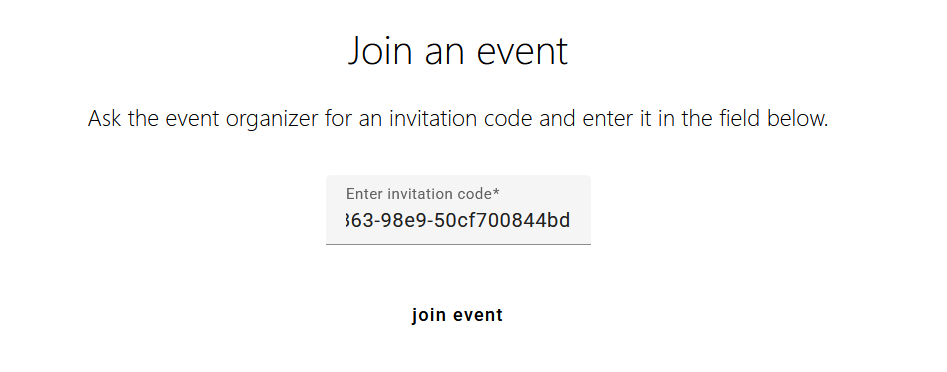
\includegraphics[width=150mm]{join_event}
\captionsetup{width=0.8\linewidth}
\captionof{figure}{A csatlakozási űrlap az elkészült alkalmazásban}
\label{join_event}
\end{center}


A szervező és a résztvevők számára látható az esemény egyedi meghívó-kódja. Ők ezt a kódot tetszőleges felületen továbbíthatják másoknak, akik ezt a kódot használva a résztvevők közé kerülnek. Az eseményhez való csatlakozáshoz regisztráció szükséges.

	\subsection{Extra mezők}

\begin{center}
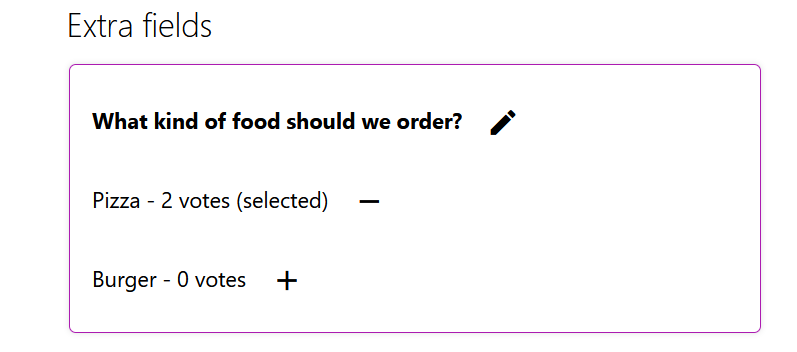
\includegraphics[width=150mm]{extra_field_food}
\captionsetup{width=0.8\linewidth}
\captionof{figure}{Egy extra mező az elkészült alkalmazásban}
\label{extra_field_food}
\end{center}

A szervező extra mezőket adhat az eseményhez. Ezekhez egy cím és a mező lehetséges értékei (továbbiakban opció) tartoznak. A mező aktuális értékét beállíthatja a szervező, vagy szavazásra is bocsájthatja azt. Emellett a szervező azt is beállíthatja, hogy a meghívottak vehetnek-e fel új opciókat az adott mezőhöz. Amennyiben a mező szavazás által dől el, minden felhasználó tetszőleges számú opcióra adhat le legfeljebb egy darab szavazatot, és azokat vissza is vonhatja. Ilyen mezők például az esemény helyszínének megadására, vagy az eseményre rendelendő étel kiválasztására szolgálhatnak. Ennél a példánál maradva, az esemény szervezője ez esetben felvehetne egy "Milyen jellegű ételt rendeljünk?" című extra mezőt, amin beállítja, hogy szavazáson dőljön el, valamint azt, hogy a résztvevők opciókat adhassanak hozzá (pl. "pizza", "hamburger").  A \ref{extra_field_food}-es ábrán ennek a mezőnek a megvalósítása látható. Az opciókhoz a '+' és '-' jelekre kattintva lehet szavazatot rendelni illetve azt visszavonni, és a fejlécen található ceruza ikonra kattintva lehet további opciókat megadni.

	\subsection{Eseménysémák használata}

Egy esemény résztvevője jogosult arra, hogy az eseményből eseménysémát készítsen. A séma tartalmazza az eseményhez rendelt extra mezőket azok tulajdonságaival és lehetséges értékeivel együtt, és alkalmas arra, hogy a használatával új eseményt lehessen létrehozni, amely extra mezői ugyanezekkel a tulajdonságokkal és értékeikben megegyező opciókkal rendelkeznek. Egy eseményhez több sémából is rendelhetünk extra mezőket, és ezek mellett továbbra is lehetőség van új mezők manuálisan történő hozzáadására.

	\subsection{Esemény adatainak véglegesítése}

Egy esemény szervezője véglegesítheti egy esemény adatait (ebbe az esemény időpontja és az extra mezők értékei tartoznak bele).  Ezután az esemény adatai nem módosíthatóak, a résztvevők pedig értesítést kapnak az esemény véglegesítéséről. A művelet visszavonható, ekkor újra módosíthatóvá válnak az adatok, az esemény résztvevői pedig erről is értesítést kapnak.

\section{Naptárak kezelése}

\begin{center}
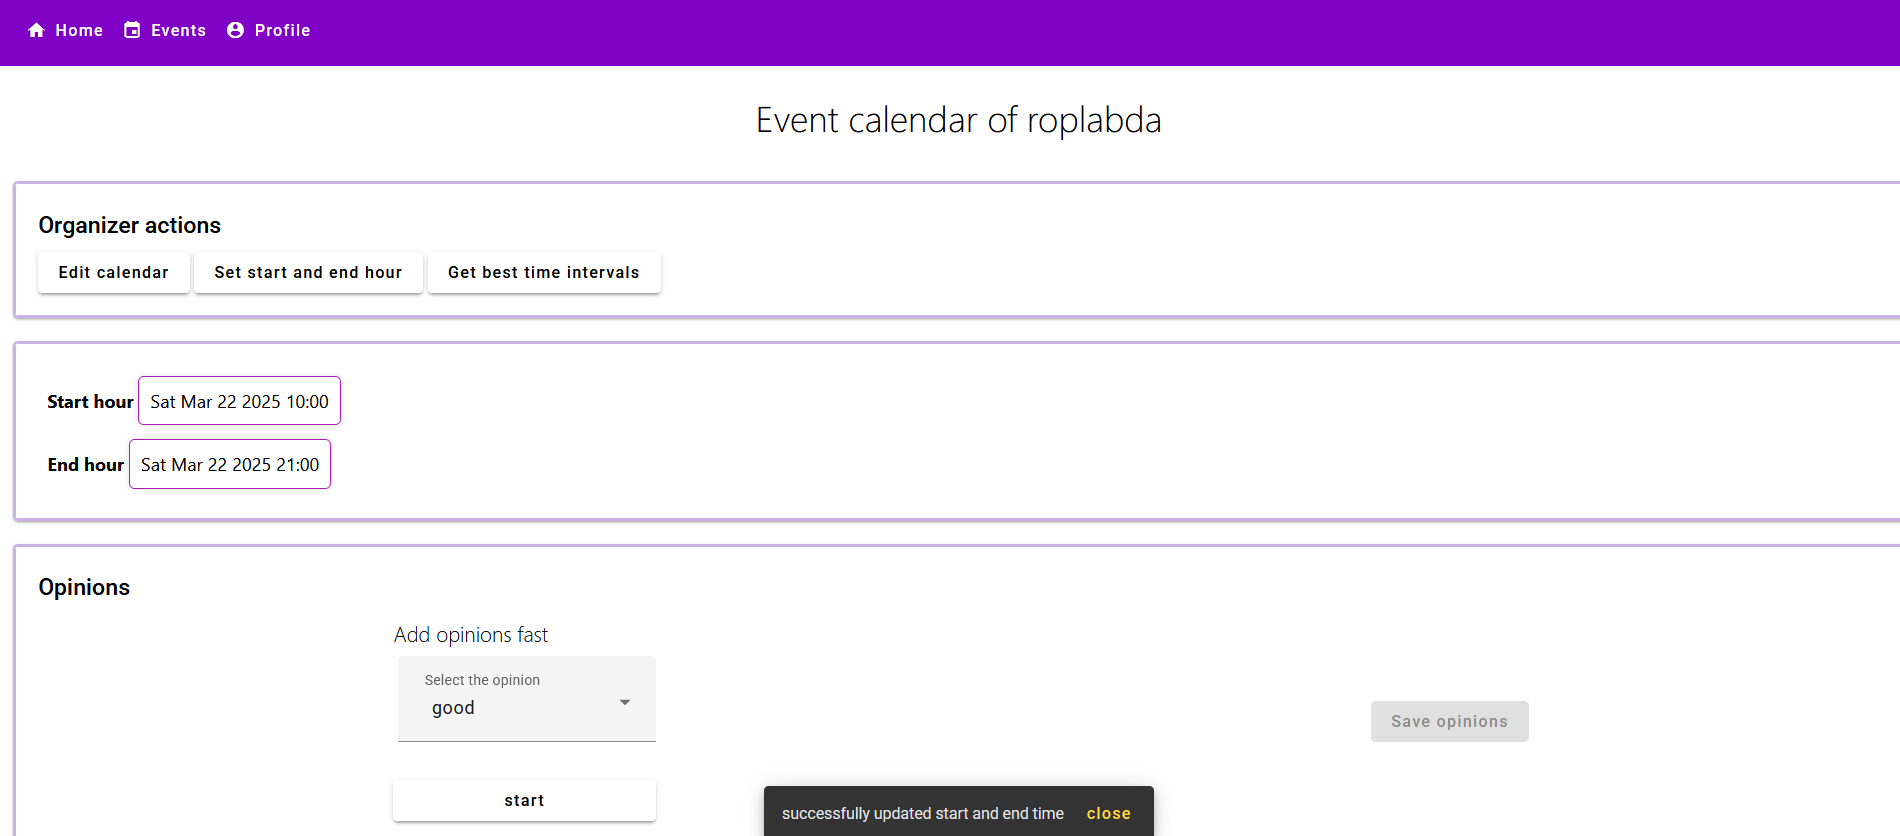
\includegraphics[width=150mm]{calendar_editor}
\captionsetup{width=0.8\linewidth}
\captionof{figure}{A naptárfelület szervezői kontrol panelje az elkészült alkalmazásban}
\label{calendar_editor}
\end{center}

A naptárfelület és a hozzá tartozó funkciók az alkalmazás legfontosabb részét alkotják, hiszen ennek a feladata, hogy segítse az esemény szervezőjét az ideális időpont kiválasztásában. A \ref{calendar_editor}-as ábrán a naptárfelület szervezői nézete látható, emellett egy résztvevői nézet is létezik, amelyről kevesebb funkció érhető el.

	\subsection{Létrehozás}

Naptár hozzáadása az időintervallum (amelynek hossza legfeljebb 60 nap lehet) és az időzóna megadásával történik. Az intervallum kezdő időpontja nem lehet a múltban, és az intervallum kezdete és vége nem lehet ugyanaz az időpont.

	\subsection{Szerkesztés}

Az esemény szervezője szűkítheti a választható időpontok körét. Az órákat és napokat letilthatja egyenként és naponta, illetve hetente ismétlődő jelleggel is. A szervező ezeket a műveleteket bármikor visszavonhatja.

	\subsection{Vélemény megadása}

Az események résztvevői (ebbe az esemény szervezője is beletartozik) minden elérhető időpontról véleményt formálhatnak. Egy időpontról megadható, hogy megfelelő, elfogadható, vagy nem megfelelő. Vélemény megadásához órákat vagy egész napokat lehet kijelölni. A vélemény rögzítése visszavonható művelet.

	\subsection{Statisztikák megtekintése}

\begin{center}
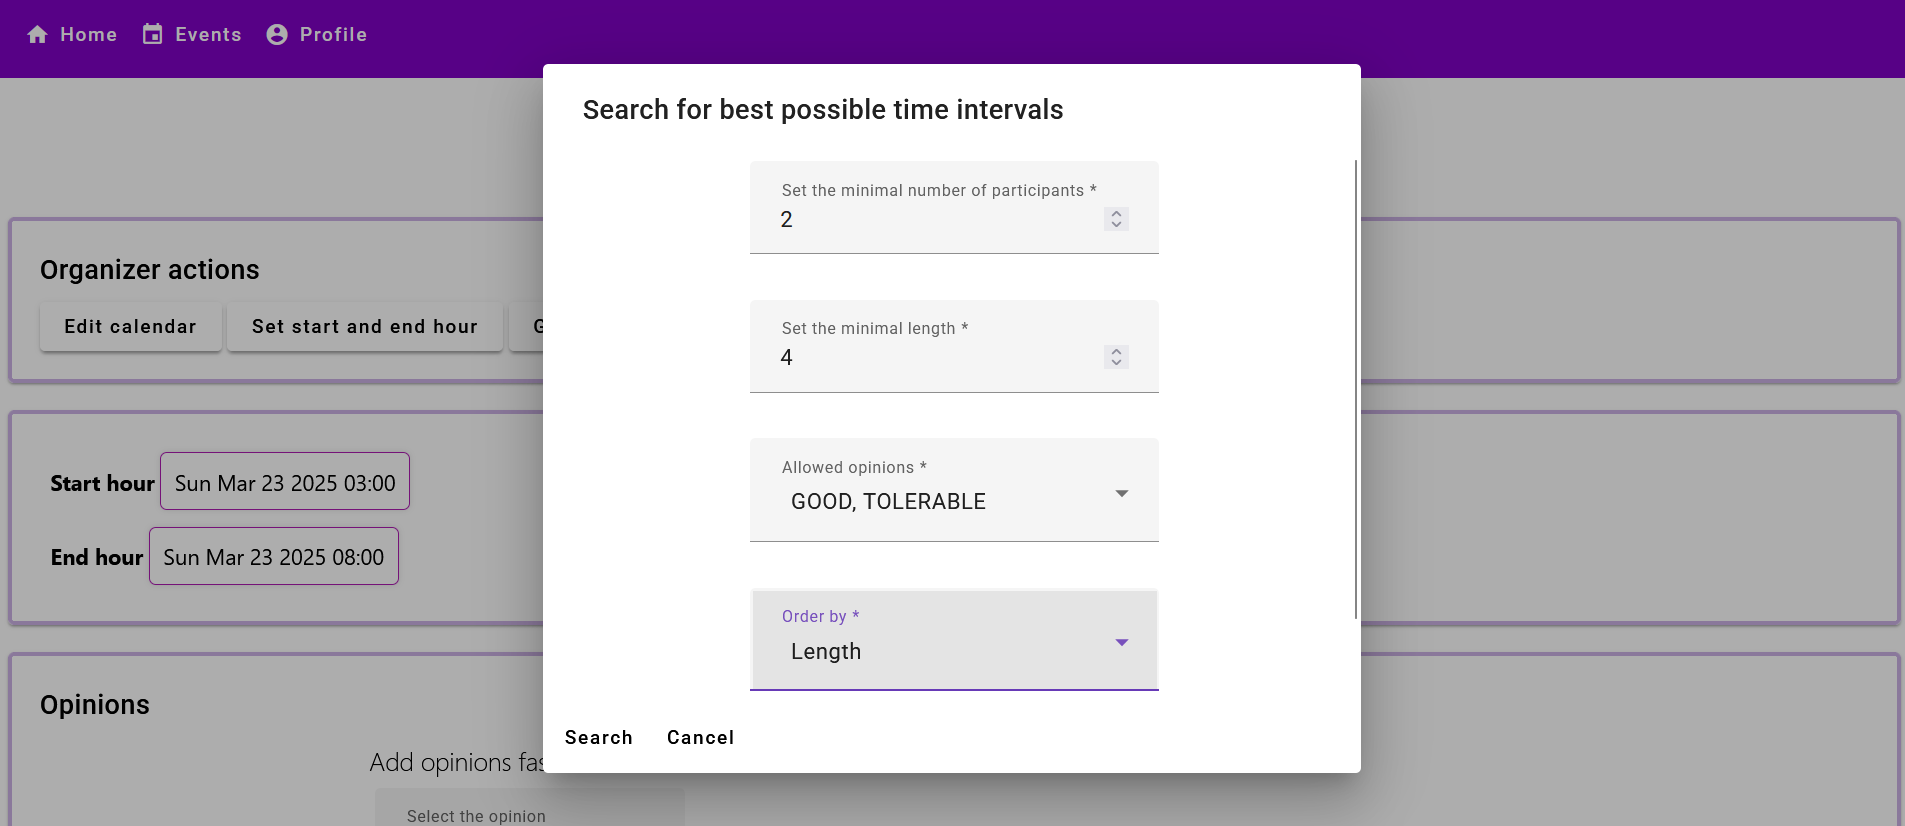
\includegraphics[width=150mm]{get_best_dialog}
\captionsetup{width=0.8\linewidth}
\captionof{figure}{Statisztikák lekérése az elkészült alkalmazásban}
\label{get_best_dialog}
\end{center}

Az események résztvevői minden időpont esetében megtekinthetik, hogy azokhoz mely felhasználók milyen véleményt rögzítettek. Az esemény szervezője átfogóbb statisztikákat is lekérhet. Egy elvárt minimális hossz és minimális résztvevőszám megadása után megtekintheti a feltételeknek megfelelő leghosszabb, illetve legnépszerűbb időpontokat. A szervező módosíthatja ezeket a lekérdezéseket, hogy azok az 'elfogadható' címkével ellátott résztvevői véleményeket is figyelembe vegyék a népszerűség kiszámolásakor, valamint az is megadható, hogy az időpontok hossza, vagy népszerűsége alapján legyen rendezve az eredmény. A két ábra kapcsolódik egymáshoz: a \ref{best_time_intervals}-ös ábrán látható lista a \ref{get_best_dialog}-es ábrán látható paraméterekkel indított időpont-keresés eredménye.

\begin{center}
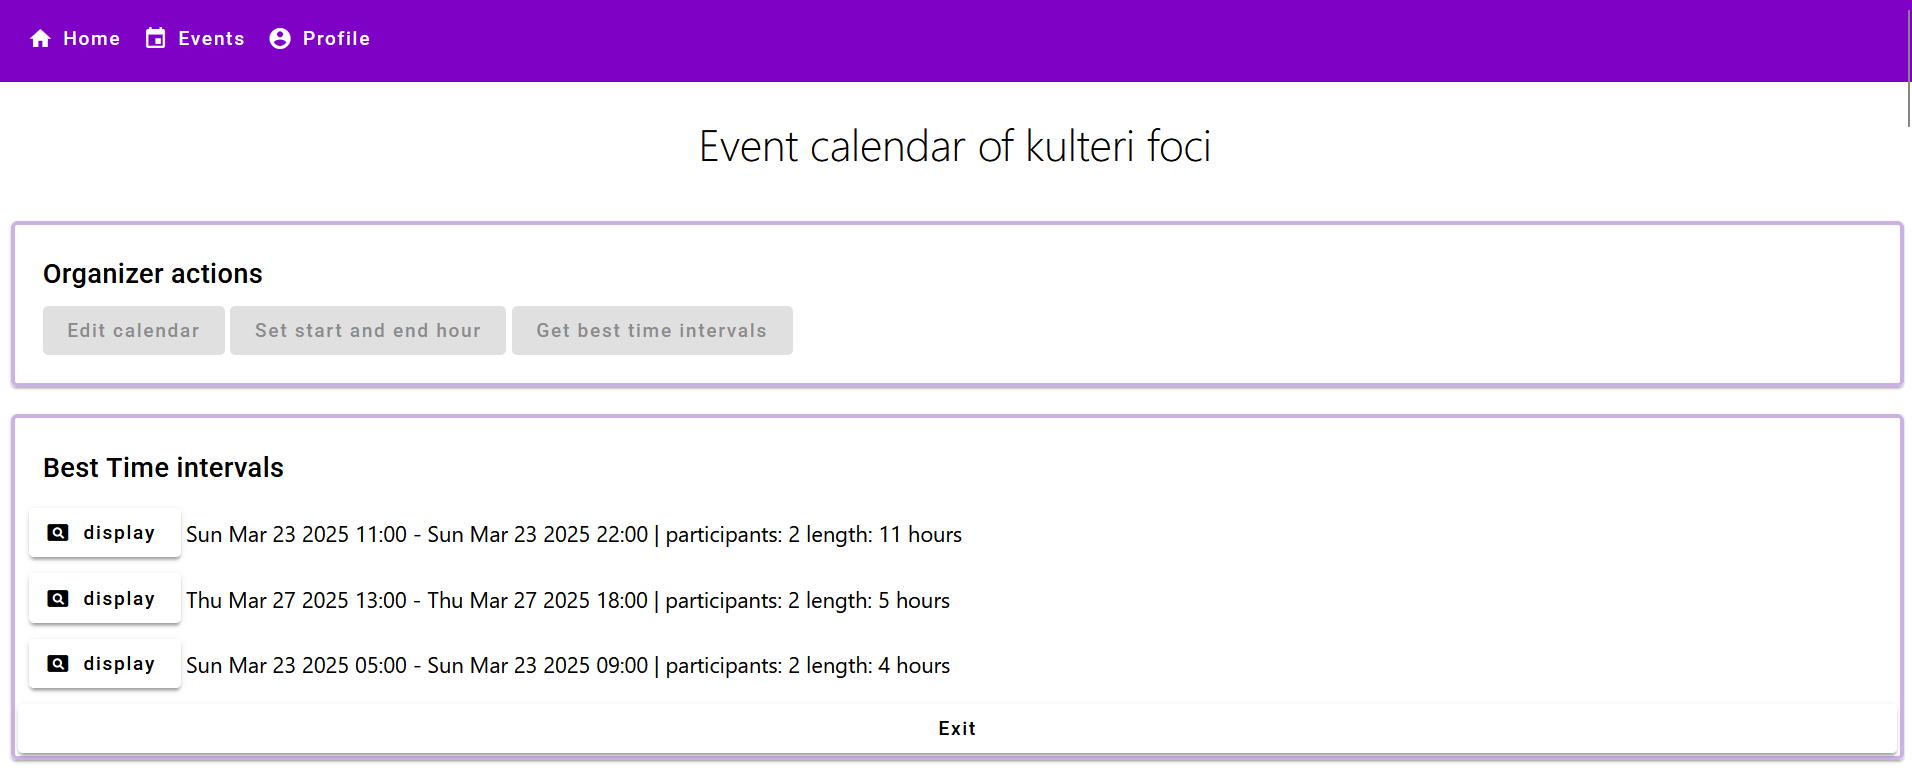
\includegraphics[width=150mm]{best_time_intervals}
\captionsetup{width=0.8\linewidth}
\captionof{figure}{Statisztikák megtekintése az elkészült alkalmazásban}
\label{best_time_intervals}
\end{center}

	\subsection{Időzónák kezelése}

Az időzóna megadása azért fontos, mert a  kiválasztható időpontok egész órák, amikből az óraátállítások esetén nem 24 van. A óraátállítások pedig különbözhetnek időzónánként. Fontos, hogy a felhasználók ne tudjanak olyan órákat kijelölni, amik nem léteznek, hiszen ez megtévesztő, és az esetleges plusz órát is jelölni kell.

\chapter{Felhasznált technológiák}

\section{Spring Boot}

A Spring Framework egy Java üzleti alkalmazások fejlesztését segítő keretrendszer. Legfontosabb funkciói közé tartozik a függőség befecskendezés és a Model-View-Controller modell (MVC) támogatása.

A backend alkalmazásomat a Spring Boot\cite{Springwebsite} használatával készítettem el. Ennek segítségével gyorsabban és egyszerűbben tudtam elkezdeni a Spring Frameworkre épülő alkalmazásom fejlesztését, mivel a Spring Boot projektek rendelkeznek alapértelmezett konfigurációs beállításokkal, nekem ezeket csak akkor kell átírnom, ha valahol az alapértelmezettől eltérő viselkedést akarok elérni. A fejlesztést InteliJ IDEA (Community Edition)\cite{IDEAwebsite} környezetben végeztem.

	\subsection{Jakarta Persistence API Hibernate ORM-el}

A Hibernate\cite{Hibernatewebsite} segítségével végeztem objektum-relációs leképezéseket a backend alkalmazásomban, ezt azonban a Java Persistence API-n (JPA)\cite{JPAwebsite} keresztül használtam. A JPA egy interfészt szolgáltat, amely segítségével a Java kódban kezelhetem a relációs adatbázisomban (esetemben a MariaDB szerveremen) tárolt adatokat. A JPA-val emellett saját natív query-ket is írtam, mivel néhány funkció megvalósításánal az adatokat egyéni módon akartam kezelni.

	\subsection{H2 In-memory DB}

A H2\cite{H2website} memórián belüli adatbázis megvalósítását az integrációs tesztjeimhez használtam. Mivel ez az adatbázis minden futtatás esetében újra inicializálódik, fejlesztés közben egyszerűbb a tesztjeimet futtatnom, hiszen így nem kell minden, a leképezendő objektumok kapcsolatait érintő változás esetén a megfelelő strukturális változtatásokat véghezvinnem az adatbázisban. Emellett általánosságban egyszerűbben kezelhető, hiszen használatához nincsen szükségem adatbázisszerverre.

\section{MariaDB}

A backend alkalmazás éles futtatása során egy MariaDB\cite{Mariawebsite} adatbázisszerverhez kapcsolódik. A MariaDB egy nyílt forráskódú, SQL alapú relációs adatbázis-kezelő rendszer (RDBMS). Más hasonló adatbázisszerverek közül azért erre esett a választásom, mert a tanulmányaim során ezt használtam a legtöbbet.

\section{Angular}

Az Angular\cite{Angularwebsite} egy Google által fejlesztett, nyílt forráskódú, TypeScript alapú keretrendszer webalkalmazások fejlesztésére. Az applikációm frontend részét ezzel valósítottam meg. A választásom azért erre esett, mert a hozzá hasonló keretrendszerek közül ezt ismerem a legjobban, és úgy ítéltem meg, hogy alkalmas modern, reszponzív felhasználói felületek létrehozására. A fejlesztést Visual Studio Code\cite{VSCwebsite} környezetben végeztem.

	\subsection{Angular Material}

A frontenden nagy számban használtam az Angular Material\cite{Materialwebsite} könyvtár komponenseit. Az Angular Material a Google hivatalos UI komponenskönyvtára, számos termékükben használják.

	\subsection{RxJs}

Az RxJs\cite{Rxjswebsite} könyvtár aszinkron műveletek kezelését segítő függvényeket és típusokat tartalmaz. A frontendemen az RxJs könyvtárban található Observable típust használtam az aszinkron API lekérdezések megvalósításához, valamint a Subject típust használtam az események megosztását végző Input és Output direktívákban.

\section{git}

A git\cite{Gitwebsite} verziókövető rendszert használtam a teljes fejlesztési folyamat során. Hogy a konzulensem is követhesse a projekt alakulását, létrehoztam egy nyilvános Github\cite{GitHubwebsite} repository-t, és oda sűrűn pusholtam a local repository commit-jait.


\chapter{Az API fejlesztése}

\begin{center}
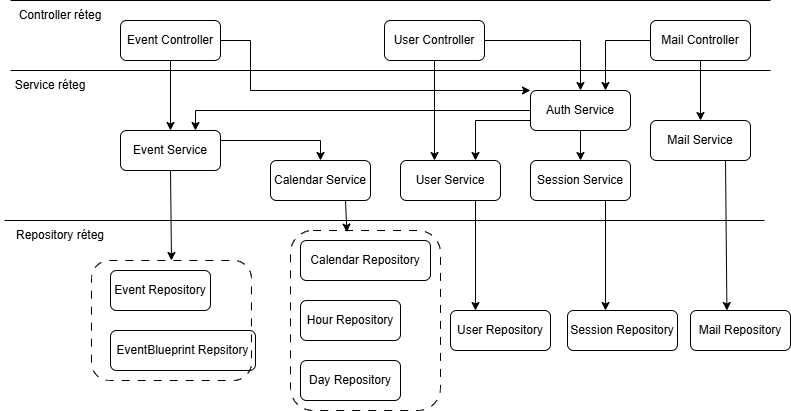
\includegraphics[width=150mm]{layers_backend}
\captionsetup{width=0.8\linewidth}
\label{layers_backend}
\captionof{figure}{A backend felépítése}
\end{center}

A \ref{layers_backend}.1-es ábrán az API felépítése látható. A Háromrétegű architektúra\cite{3layerwebsite} egy változatát, a Spring és Spring Boot projektekben gyakran használt Controller-Service-Repository architektúrát alkalmaztam, amelyben a Controller réteg feladata a bemenetek és kimenetek (a programom esetén HTTP kérések és válaszok) kezelése, a Service réteg a business logika megvalósításáért felel, a Repository réteg pedig az adatbázissal történő interakciókat végzi. Az ábrán nem tüntettem fel a Model réteget, ennek oka, hogy mivel minden Repository osztályhoz pontosan egy Model osztály tartozik, megjelenítése nem hordoz sok információt.

\section{A model réteg}

A model osztályaim egyszerű POJO-k (Plain Old Java Object). Az osztályokban sűrűn használtam a JPA objektum relációs leképzésekhez szükséges annotációit, valamint az általam szerializáláshoz használt Jackson ObjectMapper működését segítő annotációkat. Az alkalmazás további fejlesztése során gyakran használtam a Set interfészt, ezért a model osztályokban felülírtam az equals() és hashCode() metódusokat. Ezek mellett copy konstruktorokat is létrehoztam, hogy lehetőségem legyen az osztályok példányainak egyszerű másolására.

\section{A repository réteg}

Minden model osztályhoz létrehoztam egy repository interfészt, amelyeket a JPARepository interfésztől származtattam. A JPARepositoryban már az alapvető CRUD műveletek meg vannak valósítva, én azonban néhány helyen kiegészítettem ezeket új műveletekkel (például az eseményekre nem csupán az ID-jük, hanem a hozzájuk rendelt meghívó kód alapján is lehet keresni az adatbázisban). Ezeket natív query-k formájában adtam meg.

\section{A service réteg}

A service komponenseket nem az általuk használt repository-k, hanem a funkcióik szerint különítettem el, így egy service több repository-val is rendelkezhet. A service-ek között tartalmazó kapcsolat is előfordul, pédául a naptárakkal kapcsolatos műveleteket végző \textit{CalendarService} metódusai kizárólag az eseményeket kezelő \textit{EventService}-ből hívódnak meg. A service osztályokat \textit{@Transactional} annotációval láttam el, így az összes service metóduson keresztül történő művelet tranzakcióban folyik.

\subsection{AuthService}

Az \textit{AuthService} feladata a felhasználók hitelesítése és azok jogosultságainak ellenőrzése. A felhasználók bejelentkezésekor a megadott felhasználónevet veti össze az adatbázisban tárolt felhasználónévvel és megadott jelszavat az adatbázisban tárolt titkosított jelszóval a Spring Security BCryptPasswordEncoder osztály matches metódusának használatával. A sikeres bejelentkezéskor az \textit{AuthService} létrehoz egy \textit{Session} objektumot, amely a felhasználónevet (ez minen felhasználónál egyedi), a session lejáratának időpontját, valamint a session id-t tartalmazza.  A csak bejelentkezett felhasználók számára elérhető végpontokban az \textit{AuthService} metódusait használom arra, hogy az authorization header-ben érkező session id alapján a felhasználó jogosult-e a végponthoz tartozó művelet végrehajtására. A session objektum törlésre kerül, ha a felhasználó kijelentkezik, vagy ha a session lejárta után történik kísérlet annak használatára.

\subsection{EventService}

Az \textit{EventService}-ben történnek az események kezelésével kapcsolatos műveletek, a naptár kezelésének kivételével. 

Az események résztvevőinek jogosultsága van abból eseménysémát készíteni. Az \textit{EventService} ekkor az esemény összes extra mezőjét tartalmazó kollekciót JSON objektumként tárolja el az eseményséma (\textit{EventBlueprint}) adatbázistáblában egy generált ID-vel és egy felhasználó által megadott kulcsszóval együtt. A séma felhasználható új események létrehozásakor, ekkor a JSON objektumot deszerializálom, az így előállt extra mezőket a lehetséges értékeivel elmentem az adatbázisba, majd azokat az új eseményhez rendelem. Arra is ügyeltem, hogy minden felhasználó csak az általa létrehozott sémákhoz férhessen hozzá, ehhez egy insertUser tulajdonságal kellett kibővítenem az \textit{EventBlueprint} model osztályt.

\subsection{CalendarService}

A naptárak kezelése a \textit{CalendarService}-en keresztül történik.

Az óraátállítások fennállásának ténye nehézségeket okozott, hiszen nem akartam lehetővé tenni, hogy a naptár felületen nem létező órák elérhetőek legyenek (ilyenek azok az órák amelyeket a tavaszi óraátállítás során kimaradnak), és azt sem, hogy kimaradjanak olyan órák, amelyek a megszokott 24 órán kívül vannak (ezek az őszi óraátállítás során betoldott órák). Mivel az óraátállítások időzónánként eltérnek, a naptárak létrehozásakor paraméterben elvárom az időzóna megadását is. Ezután az időzóna segítségével Java ZonedDateTime objektumokat készítek a naptár kezdő és záró időpontjából, és a ZonedDateTime metódusainak segítségével generálom le a közöttük levő órákat. Ily módon a két időpont közötti összes óra benne lesz a naptárban, és egyetlen kimaradó órát sem fog tartalmazni.

Az legjobb időpontok megtalálása az egyik legfontosabb funkciója az alkalmazásnak. Ez a \textit{getBestTimeIntervals} függvényen keresztül történik, amely négy paramétert vár: a naptárat, a résztvevők minimális számát, az időpontok minimális hosszát, és az elfogadott felhasználói véleménytípusok listáját. A függvény minden órához az ettől az órától kezdődő, a paraméterekben megadott minimális hossznak és minimális résztvevőszámnak megfelelő időpontokat rendeli. Egy ilyen időszak esetében az számít részvevőnek, aki az időszak összes órájára a paraméterben megadott véleménytípusok egyikét választotta.

Az algoritmus a következőképpen működik: az eseményhez tartozó összes óra objektumon végigiterál, és egy listába összegyűjti az egyes óráktól kezdődő összes olyan időpontot, amely a megadott feltételeknek megfelel. A függvényben, az adott órától kezdődő időpontokat keresi, egy halmazban tárolom azokat a felhasználókat, akik számára visszajelzésük alapján megfelel az óra. Ezután végigiterálok az ezt követő órákon, és frissítem a halmazt oly módon, hogy az csak azokat a felhasználókat tartalmazza, akiknek az éppen vizsgált óra is megfelelő. Amennyiben a halmaz szűkült és már legalább annyi órát vizsgáltunk, mint amennyi a paraméterben megadott minimális hossz, létrehozok egy időpont objektumot a kezdő óra, a hossz, valamint a felhasználói halmaz megadásával, és azt felveszem a visszaadandó időpontok listájába. Ha a halmaz mérete a paraméterben megadott minimális résztvevői szám alá csökken, kilépek a ciklusból, és a következő órára kezdem el keresni az időpontokat.

Az időpontokat tartalmazó lista hossza legrosszabb esetben
\begin{equation} \label{eq:eq1}
\sum_{n=1}^{a*24+1} {n}
\end{equation}
elemet adhat vissza, ahol \textit{a} az esemény naptárjához rendelt napok száma, ez legfeljebb 60 lehet, ez alapján a visszaadott lista maximális mérete
\begin{equation} \label{eq:eq2}
 \sum_{n=1}^{1441} {n} = 1 038 961
\end{equation}
, ennyit nem szeretnék a frontenden feldolgozni. Ezért a \textit{getBestTimeIntervals} függvényt használja a \textit{getLongestTimeIntervals} és a \textit{getMostPopularIntervals} függvény, amelyek a hossz, illetve a népszerűség alapján rendezik az eredmények listáját, és csak a legjobb tizet adják vissza. A REST végpontokból csak ez a két függvény érhető el.

\subsection{MailService}

A felhasználóknak küldött rendszeren belüli üzenetek kezelését végzi.

A felhasználók üzeneteket kapnak az esemény lezárásáról, illetve az eseményt lezáró művelet esetleges visszavonásáról. Az események lezárásaról tájékoztató üzenet tartalmazza az eseményhez tartozó mező-érték párokat (ebbe az esemény kezdete és vége is bele tartozik, amennyiben naptárt is rendelt a szervező az eseményhez). Ezeket egyszerű szövegként nehéz értelmezni, ezért ezt formázott szövgként táblázatos formában terveztem megjeleníteni. Mivel a frontend oldalon nem terveztem módosításokat végrehajtani a backendről érkező levéleken, ezért a formázott üzenetet a backenden készítettem el, HTML formátumban. Mivel nem találtam az igényeimnek megfelelő Java könyvtárat, ezért elkészítettem a \textit{HTMLWriter} osztályt amelyben HTML elemeket előállító statikus metódusokat írtam. A formázott levelek frontend oldalon történő kezeléséről lejjebb értekezem.

\section{Controller réteg}

A controller osztályok szintén funkciók szerint különülnek el, ezért mindegyik tartalmaz hivatkozást a releváns service komponensére, valamint az \textit{AuthService}-re, amely a védett végpontok esetében végzi el a felhasználók autorizációját. Minden controller osztályhoz egy útvonal, a REST végpontokat megvalósító metódusaihoz pedig egy-egy alútvonal tartozik.

\subsection{Szerializálció, deszerializáció}

A model osztályaim példányait nem lehet egy-az-egyben JSON objektumokká alakítani. Az egyik probléma az osztályok közötti körkörös hivatkozások fennállása. Ezt tartalmazó kapcsolatok esetén úgy oldottam meg, hogy a tartalmazott osztályban Jackson \textit{@JsonIgnore} annotációval tiltottam meg a tartalmazó osztály kapcsolódó példányának szerializálását, egyenrangú kapcsolatok esetén pedig azt teljesen ignoráltam a szerializáció során, a kapcsolat résztvevőit csak külön lekérések által tettem elérhetővé. Egyes osztályok esetén fennállhat az igény arra, hogy egyes tulajdonságait csak deszerializálni lehessen. Ilyen például a felhasználó osztály jelszó mezeje, hiszen, bár titkosítva van, ezt nem célszerű a frontend felé továbbítani, ellenben a deszerializálására szükség lehet a regisztráció során. Ezt úgy oldottam meg, hogy az adott tulajdonságot \textit{@JsonProperty(access = JsonProperty.Access.WRITE\_ONLY)} annotációval láttam el.

\section{Kivételkezelés}

Külön kivételosztályokat hoztam létre az események, felhasználók, naptárak kezelése, illetve felhasználók autorizációja során keletkező kivételeknek. A speciálisabb kivételosztályokat ezekből az ősosztályokból öröklődtettem. A controllerek működése során keletkező, el nem kapott kivételek részére létrehoztam egy \textit{ControllerAdvice} interfészt implementáló globális kivételkezelő osztályt. Ebben megadtam, hogy a keletkezett kivétel függvényében a visszaküldendő válasz milyen üzenetettel és státuszkóddal rendelkezzen.

\section{Tesztelés}

Minden service és controller komponenshez saját tesztosztályt hoztam létre, amelyeket az absztrakt \textit{EowaIntegrationTest} osztályomból származtattam.  A tesztekhez egy properties fájlt is létrehoztam, ebben megadtam, hogy a tesztek ne a MariaDB adatbázisomat, hanem egy memórián belüli H2 adatbázist használjanak. A service-ekhez tartozó tesztek írása során törekedtem a teljes tesztlefedettségre, a controller-ekhez tartozó tesztek esetében csak annyi tesztet írtam, amennyiből megállapítható, hogy a szerializálás, a deszerializálás, és a kivételek kezelése megfelelő módon történik. A tesztlefedettség méréséhez a JaCoCo\cite{Jacocowebsite} Maven plugin-ját használtam, a teljes coverage report (a \ref{jacoco}-es számú melléklet)  és service réteg coverage report-ja (a \ref{jacocoservice}-es számú melléklet) a mellékletek között található. Ezeken látszik, hogy a service rétegben az utasítások lefedettsége 96\%, a metódusok lefedettsége pedig 100\%. A controllereket MockMvc használatával teszteltem. A teszteseteket az "3 A"\cite{3Awebsite} (Arrange, Act, Assert) szabály szerint készítettem el, azaz először elkészítettem a tesztesethez szükséges objektumokat, ezután elvégeztem a vizsgálandó műveletet, majd ellenőrzöm, hogy az elvárt eredményt sikerült-e elérni.

\section{Védelem}

	\subsection{CORS}

A Spring Security-ben lehetőség van saját CORS, azaz a Cross-origin Resource Sharing\cite{Corswebsite} configuráció megadására. Ebben megadható, hogy a szerver mely domainekről fogad kéréseket, és azt is, hogy azok esetében mely kérés metódusokat és header-öket engedélyezi. A konfigurációmban kizárólag azt az útvonalat engedélyeztem, amelyen a frontend alkalmazásom érhető el, arról viszont az összes metódust és header-t elfogadtattam.


	\subsection{CSRF elleni védekezés}

A CSRF a Cross Site Request Forgery rövidítése. A CSRF lényege, hogy az egyik oldalra bejelentkezett felhasználó egy másik oldalon elrejtett űrlapon keresztül, tudta nélkül küld kérést a szerver felé\cite{Infbiztwebsite}. Ennek nagy a kockázata session cookie-k használata esetén, mivel a böngészősütikhez más oldalak is hozzáférnek, ezért a session id-t nem sütikben, hanem az authorization headerben várják az alkalmazás REST végpontjai, a frontend oldalon pedig a localstorage-ben tárolom azt, így más oldal nem férhet hozzá.


	\subsection{XSS elleni védekezés}

Mivel az esemény adatainak véglegesítéséről küldött üzenetet HTML formában továbbítom a frontendre, és ebben felhasználók által megadott szövegek (az esemény neve, leírása, az extra mezők neve és értékei) is szerepelnek, ez alkalmas lehet kártékony szkriptek más felhasználókhoz történő eljuttatására. Az efajta támadást DOM alapú XSS-nek, azaz Cross Site Scripting-nek nevezzük\cite{Infbiztwebsite}. Hogy ezt megelőzzem, a felhasználók által megadott szöveget csak azután használom fel arra, hogy a HTML tagek közé illesszem, hogy azokban escape-elem a speciális karaktereket.

	\subsection{SQLi}

Az SQLi\cite{Infbiztwebsite2}, azaz SQL befecskendezés esetén a támadó az SQL query-kben felhasznált, felhasználói bemenetből származó adatok ellenőrzésének és megfelelő feldolgozásának hiányát használja ki oly módon, hogy azok segítségével manipulálja az ezeket felhasználó query-ket. A natív query-k esetében a felhasználótól érkező adatokat nevekkel ellátott paraméterekként adtam át, ezek a Hibernate által  \textit{prepared statement}-ekben kerülnek felhasználásra, így védettnek minősülnek\cite{hibernatewebsite2}. A natív query-k mellett a JPARepository interfész metódusait használtam, amelyeknek Hibernate-es megvalósításai szintén paraméter kötést alkalmaznak.

\chapter{A frontend fejlesztése}

\section{Model réteg}

Az egyes backend oldali model osztályoknak megfelelő TypeScript interfészeket írtam, hogy megfelelően szerializálhassam és deszerializálhassam őket. Ezek nem tekinthetőek viewmodel\cite{Viewmodelwebsite} osztályoknak, hiszen nem csupán a megjelenítés a céljuk, pédául az id tulajdonságokat is tartalmazzák.

\section{Service réteg}

Az \textit{ApiService}-ben írtam meg a fetch API-t\cite{Fetchwebsite} használva a backend felé HTTP kéréseket küldő metódusokat, valamint a kéréshez tartozó header-öket is itt állítom össze (utóbbiakból a legfontosabb az authorization header, amelybe az aktuális felhasználó session információi kerülnek). A többi service osztályba pedig az \textit{ApiService}-t injektáltam, így az összes kérés rajta keresztül zajlik.  Mivel az üzleti logika kizátólag a backend oldalon található, az összes service metódus egyetlen, az API felé küldött kérésből és a válasz feldolgozásából áll.

\section{Pipe-ok}

Az angular Pipe-ok\cite{Pipewebsite} segítségével egyszerűen lehet a template fájlokban JS objektumokat megjeleníthető formába alakítani. Én több ilyet is létrehoztam, például egy pipe segítségével jelenítem meg a pontos dátumot a naptárfelületen. Itt a pipe transform metódusa a naptár objektumot és az óra sorszámát kapja meg, majd ezek segítségével adja vissza a pontos dátumot leíró sztringet, vagy az "end of the event" szöveget.

\section{Navigáció az oldalon}

A komponensek közötti navigáció megvalósításához azokba az Angular Router service-t\cite{Routerwebsite} injektáltam, amely az app.routes fájlban tárolt útvonalak és az azokhoz társított komponensek és guard függvények segíségével végzi el a szükséges műveleteket. Egyes esetekben query paramétereket is használtam, ezeket a komponensekbe injektált ActivatedRoute segítségével kértem le. Erre példa ViewEvent komponens, amely esetén a megjelenítendő esemény id tulajdonságát query paraméter formájában továbbítom a komponenshez tartozó útvonalra navigáláskor.

\section{Fő komponensek}

	\subsection{Dialógusablak}

\begin{center}
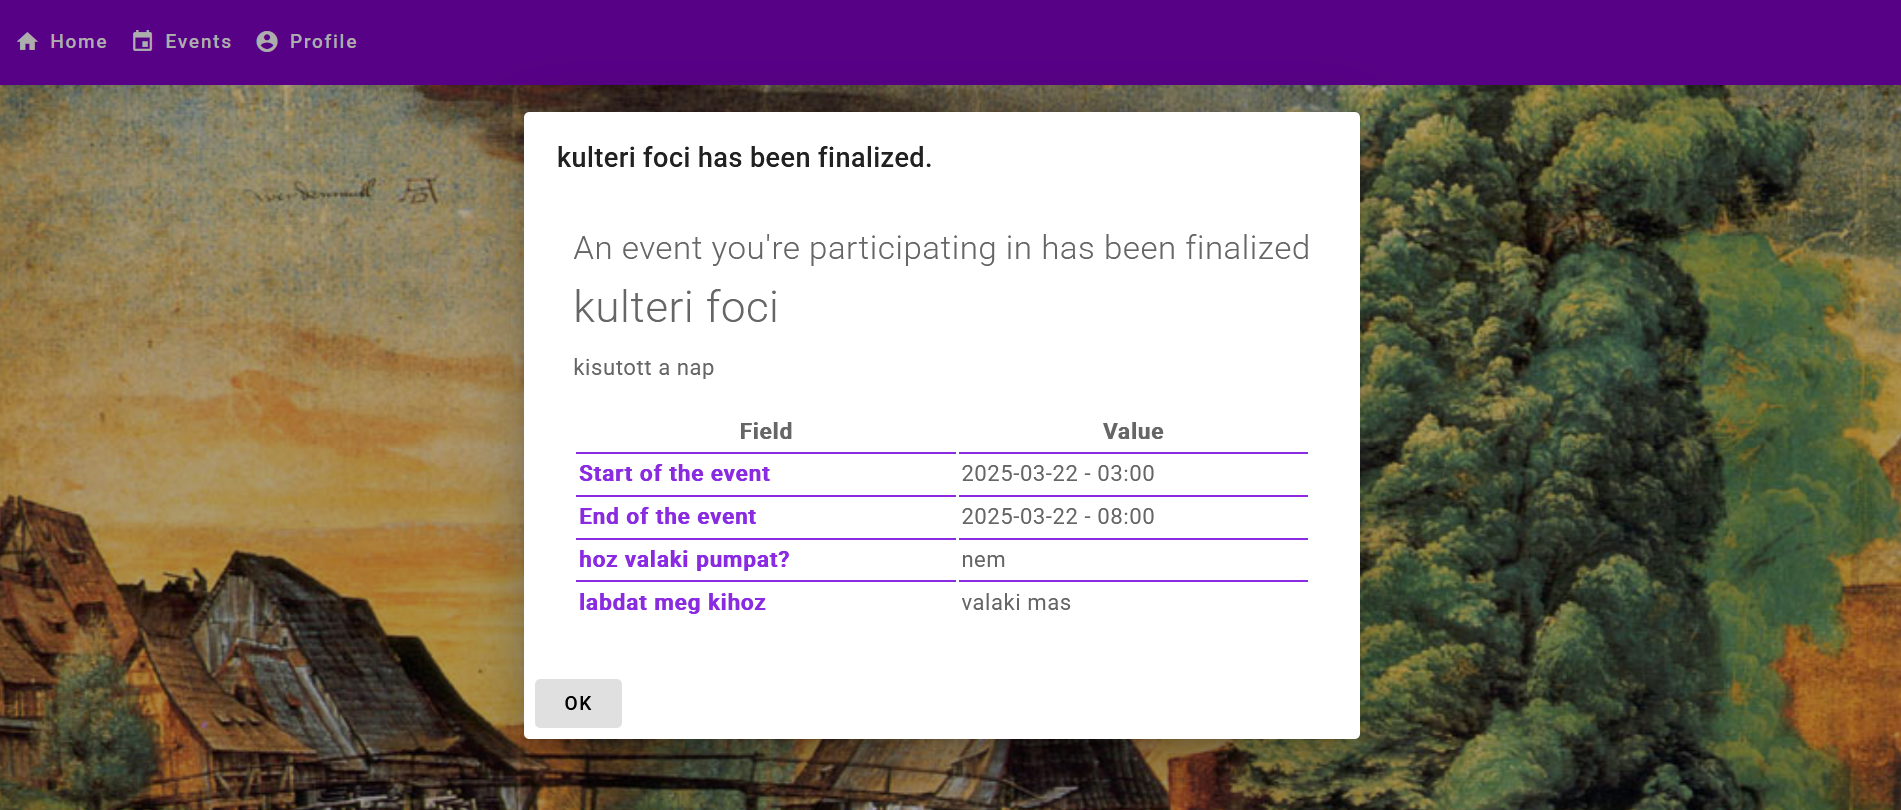
\includegraphics[width=150mm]{notification}
\captionsetup{width=0.8\linewidth}
\captionof{figure}{Értesítés esemény lezárásáról a dialógusablak komponens használatával}
\label{notification}
\end{center}

Saját dialógusablak komponenst hoztam létre, amely alkalmas formázott és formázatlan üzenetek megjelenítésére is. A formázott szöveg megjelenítését az események lezárultát tudtul adó üzenetek esetén használom, hiszen ezek táblázatokat is tartalmaznak.  A HTML formában megadott üzeneteket egyirányú kötéssel a dialógus komponens InnerHTML tulajdonságához rendeltem, és a stílust is a frontend oldalról adtam meg, hogy azt ne kelljen redundáns módon az adatbázisban tárolni minden üzenet rekordban. Az \ref{notification}-es ábrán egy ilyen módon előállított üzenet látható.

	\subsection{Naptárfelület}

\begin{center}

\includegraphics[width=150mm]{view_calendar_structure}
\captionsetup{width=0.8\linewidth}
\captionof{figure}{A naptárfelület felépítése}
\label{view_calendar_structure}
\end{center}

A naptárfelület több standalone komponensből tevődik össze, ezt foglalja össze az \ref{view_calendar_structure}-es ábra. A \textit{ViewCalendarComponent}-en belül az egyes napokhoz, és azokon belül az órákhoz külön komponens tartozik. Mivel az \textit{HourComponentben} és a\textit{ DayComponentben} keletkező változtatásokat az azokat magában foglaló \textit{ViewCalendarComponentben} összesítem és azokat egy megerősítő felhasználói interakció után egyetlen HTTP üzenetben küldöm el az API-nak, az \textit{EventService}-t csak a \textit{ViewCalendarComponent}-ben injektáltam. A \textit{ViewCalendarComponentben} keletkező események az összes gyerek komponensre hatással vannak, a gyerek komponensekben keletkező eseményeket pedig a \textit{ViewCalendarComponent} összesíti a fent említett módon, ezért a \textit{DayComponent}-ben és az \textit{HourComponent}-ben Input és Output direktívákat alkalmaztam, hogy az adatok mindkét irányban megfelelő módon áramoljanak. A \textit{ViewCalendarComponentben} keletkező eseményre példa a szerkesztői nézetre váltás, erről a nap és óra komponenseknek is értesülniük kell, mivel szerkesztői nézetben megváltozik a viselkedésük.

\section{Űrlapok reaktív módon történő kezelése}

\begin{center}
\begin{tabular}{cc}
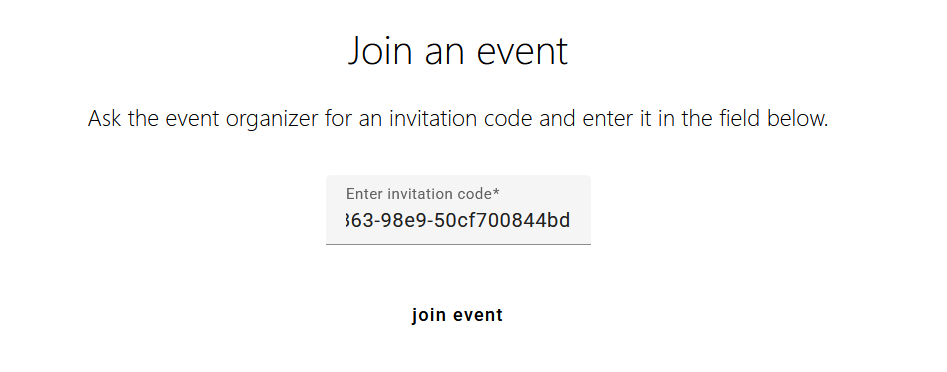
\includegraphics[width=70mm]{join_event}
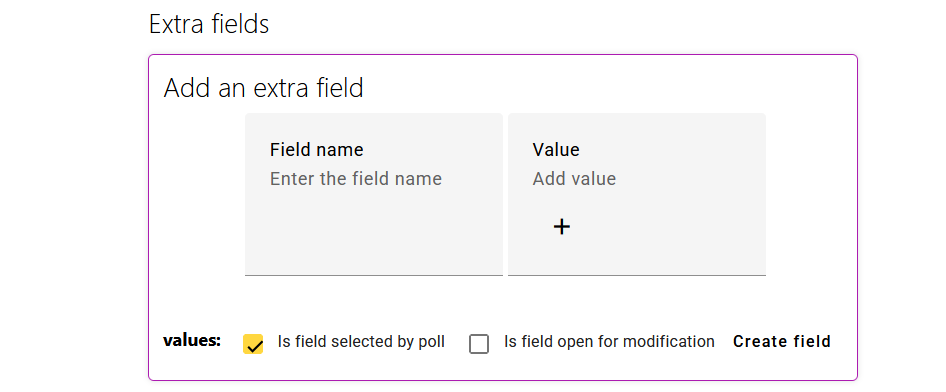
\includegraphics[width=70mm]{extra_field_form}
\end{tabular}
\captionsetup{width=0.8\linewidth}
\captionof{figure}{Példa egyszerű és összetett űrlapra}
\end{center}

Az egyszerű, egyetlen input mezőből álló és frontend oldali validációt nem igénylő űrlapokat kétirányú adatkötéssel dolgoztam fel, az összetettebbeket azonban a ReactiveFormsModule\cite{ReactiveFormswebsite} segítségével alkottam meg. Az űrlapokhoz FormGroup-okba gyűjtött FormControl objektumokat rendeltem, amelyekhez validációs függvényeket is írtam, ahol a ReactiveFormsModule előre megírt függvényei nem voltak elegendőek. Erre példa a függvény, amelyet annak ellenőrzésére használtam a  \textit{SignUp} komponensben, hogy a felhasználó által a regisztráció során megadott két jelszó megegyezik-e.

\section{UX, UI}

	\subsection{Progress indicator}

\begin{center}

\includegraphics[width=75mm]{progress_indicator}
\captionsetup{width=0.8\linewidth}
\captionof{figure}{A progress indicator komponens}
\end{center}

Létrehoztam egy saját progress indicator komponenst, amely segítségével jelzem a felhasználó felé, ha a kért útvonalhoz tartozó komponens még nem tölthető fel adatokkal, mivel azoknak az API-tól való lekérése éppen most zajlik. Ezzel helyettesítem az adott komponens tartalmát annak inicializálásától kezdve az API-tól érkező válaszig (akkor is, ha az hibát jelez). Ezt természetesen nem alkalmazom azokban az esetekben, amikor a komponens megjelenítendő adai rendelkezésre állnak, és az API-val történő kommunikácó befejeztét nem kell megvárnia a felhasználónak, hogy más műveletek végrehajtson.

	\subsection{Guard-ok}

Az Angular-ban a canActivate guard-ok olyan függvények, amelyek a CanActivateFn\cite{Guardwebsite} interfészt implementálják, és segítségével eldönthető, hogy a felhasználó navigálhat-e egy adott al-útvonalra az oldalon belül. Használatuknak jellegzetes esete guard-ot rendelni azokhoz az útvonalakhoz, amelyeket csak bejelentkezett felhasználók használhatnak. Ez UX funkció, hiszen az ilyen útvonalakhoz rendelt komponensekből olyan funkciók is elérhetőek, amelyekre a választ a szerver vissza fogja utasítani, ha nincs bejelentkezve a felhasználó, ennek előfordulása egy guard használatával elkerülhető. Én is írtam egy ilyen függvényt, amelybe a  \textit{UserService}-t injektáltam, hogy annak  \textit{getCurrentUser} metódusa segítségével eldönthesse, jogosult-e a felhasználó az útvonal aktiválására.

	\subsection{Folytonos színátmenet style binding segítségével}

\begin{center}
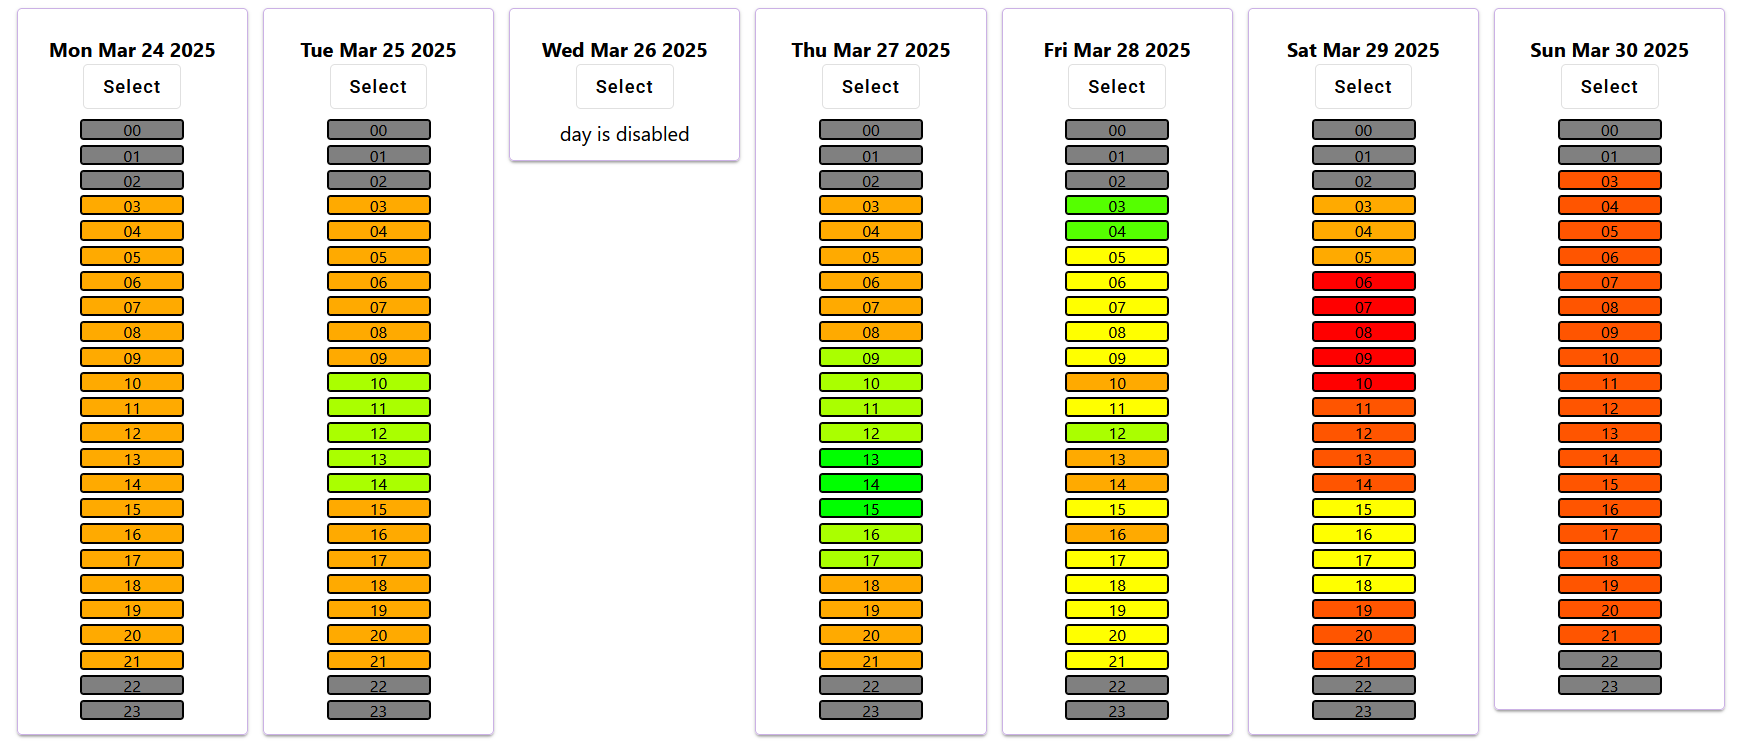
\includegraphics[width=160mm]{week_view}
\captionsetup{width=0.8\linewidth}
\captionof{figure}{Az időpontok népszerűségének megjelenítése színek segítségével}
\label{week_view}
\end{center}

A naptárfelületen színek segítségével jelenítem meg, hogy az egyes órák mennyire népszerűek a résztvevők körében. Ahogyan az \ref{week_view}-ös ábrán is látszódik, a legtöbb felhasználónak megfelelő órák a legélénkebb zöld színnel, a legkevesebb felhasználónak megfelelő órák pedig a legélénkebb piros színnel vannak megjelölve. Az óra komponensben létrehoztam egy függvényt, amely annak népszerűségét a felhasználói vélemények alapján egy nulla és egy közötti szám formájában adja vissza. Ennek függvényében akartam a komponensek háttérszínét a pirostól a zöld színig terjedő skálán elhelyezni, ezért egy új tulajdonságot vezettem be a komponensben, amelyben a háttérszínt RGB formátumban tároltam. A kék összetevőt nullára állítottam, a zöld összetevőt a népszerűséggel egyensen arányos módon, a piros összetevőt pedig a fordítottan arányos módon állítottam be. A tulajdonságot pedig a template fájlban stíluskötéssel állítottam be háttérszínnek.

	\subsection{Canvas Angularban}

Az óra komponensekre kattintva megjelenik egy dialógusablak, amely információkkal szolgál az adott órához tartozó véleményekről. Itt egy egyszerű diagramot is elhelyeztem, hogy az információk könnyebben feldolgozhatóak legyenek. Ezt egy beépített Canvas segítségével alkottam meg. A komponens fájlban egy ViewChild dekorátorral konfigurált HTMLCanvasElement típusú ElementRef segítségével tudok a template fájlban megadott canvas-re hivatkozni.

\section{Aszinkron programozási megoldások}

Az aszinkron műveletekhez az RxJs könyvtár eszköztárát használtam. Hogy ez mindenhol egységes legyen, a Promise-okat visszaadó függvények eredményeit RxJs Observable objektumokká alakítottam, ilyen az összes, HTTP kérést tartalmazó service függvényem, hiszen ezek a fetch API-t használják. Az RxJs Subject típusát az események megosztását végző Input és Output direktívákban alkalmaztam.
 
\chapter{Továbbfejlesztési lehetőségek}

Az alkalmazást a fejlesztés folyamán csak a saját eszközömöm futtattam, logikusnak tűnik következő lépésként egy alkalmas szerverszolgáltatás igénybevétele, esetleg saját szerver felállítása, amely segítségével a webalkalmazás a világhálón keresztül elérhetővé tehető más eszközök számára is.

Az egyik lehetőség a továbbfejlesztésre a JWT\cite{JWTwebsite} (Jason Web Token) használata az autorizációs folyamatokra. A jelenlegi megoldásom, bár a localstorage-ben tárolt json objektum segítségével zajlik, nem nevezhető jwt-nek, mivel az autorizáció a benne tárolt session id alapján történik, aminek hitelességét a backend oldalon kell lellenőrizni, és nem egy digitális aláírás segítségével.

Az alkalmazás reszponzivitása javítható, jelen állapotban például mobilról nehezen használható. Emellett a felhasználói felület akadálymentesítésével is érdemes lehet foglalkozni.

Az értesítések nagyobb valószínűséggel juthatnak el a felhasználókhoz, ha megvalósítanám, hogy az értesítéseket a megadott emal-címükre is megkapják a felhasználók.

\chapter{Hasonló alkalmazások}

Bár én a projekt megkezdése előtt nem hallottam róla, az alkalmazás írása közben többen felhívták rá a figyelmemet, hogy hasonló célra készült alkalmazások már léteznek, ezért ezeknek utánanéztem, hogy összehasonlíthassam őket a saját megoldásommal. A legtöbben a Doodle alkalmazást említették, emellett a ClickUp, valamint a WhenAvailable merült még fel. Az alábbiakban az alkalmazásomat a Doodle\cite{DoodleWebsite} ingyenes változatával vetem össze.

\section{Doodle}

A Doodle-ban több, az enyémhez hasonló megoldás is van, például az eseményhez csatlakozás egy megosztott linken keresztül történik, valamint itt van egy esemény véglegesítő művelet, amelyről a résztvevők értesítést kapnak.  További hasonlóság, hogy az egyszerű "megfelel" mellett az "amennyiben nincs más lehetőség" válasz is elérhető. Különbség, hogy ebben csak előre megadott, konkrét időpontokra lehet jelentkezni, valamint az is, hogy az esemény más tulajdonságait (pédául a helyszínt) a szervező nem teheti szavazás tárgyává. Különbség az is, hogy a Doodle-ben regisztráció nem szükséges, az értesítéseket az eseményhez társított email-címükre kapják a felhasználók. A doodle-ben a véglegesítési művelet nem vonható vissza, és mivel extra mezőket nem lehet az eseményekhez társítani, következtetésképp azokból eseménysémákat sincs lehetőség létrehozni. A legtöbb különbség abból adódik, hogy a Doodle-t elsősorban előre meghatározott időponttal rendelkező, szigorú keretek között megvalósuló meeting-ek megszervezésére készítették, míg az én alkalmazásom inkább arra hivatott, hogy egy adott baráti társaság találkozóinak rugalmas szervezését segítse.

\chapter{Összefoglalás}

Az alkalmazás legfontosabb funkcióit mind megvalósítottam. A használatával eseményeket lehet létrehozni, lehetőség van azok konfigurációjára és sokszorosítására. Az eseményekhez más felhasználók is adhatók, az általuk adott visszajelzésekről könnyen értelmezhető statisztikákat kap az esemény szervezője. Az események adatainak véglegesítéséről a felhasználók alkalmazáson belüli üzenetben értesülnek. Ám az alkalmazás még nem teljes, számos felhasználói élményt javító funkcióval kibővíthető.

A fejlesztés során a tesztelésre nagy gondot fordítottam, külön tesztelési környezetet hoztam létre, amely a produkcióstól eltérő adatbázis kapcsolattal rendelkezett. Valahányszor új funkciókkal bővítettem ki az alkalmazást, teszteket is írtam azokhoz, így sikerült nagy tesztlefedettséget elérnem.

Az alkalmazás készítése során új ismeretekre is szert tettem, elsősorban a biztonsági megfontolások terén, az SQL befecskendezés elleni védekezési módok ismertek voltak számomra, a CSRF és XSS támadások elhárítására szolgáló megoldások azonban újak voltak számomra.

Bár léteznek már hasonló célra készült alkalmazások, úgy hiszem, hogy elsősorban a rugalmassága miatt az alkalmazásom egy létező igényt elégít ki.

\newpage

\bibliographystyle{unsrtdin}
\bibliography{mate_koncz} 

\newpage
{\Huge \bf Nyilatkozat}

 \addcontentsline{toc}{chapter}{Nyilatkozat}

\vspace{2 cm}

Alulírott, Koncz Máté, Programtervező Informatikus szakos hallgató, kijelentem, hogy a szakdolgozatban ismertetettek saját munkám eredményei, és minden felhasznált, nem saját munkából származó eredmény esetén hivatkozással jelöltem annak forrását. 


\begin{flushleft}
\vspace*{1cm}
Szeged, \today
\end{flushleft}

\begin{flushright}
 \vspace*{1cm}
 \makebox[7cm]{\rule{6cm}{.4pt}}\\
 \makebox[7cm]{\emph{Koncz Máté}}
\end{flushright}

\pagebreak

\newpage
\section*{Mellékletek}

 \addcontentsline{toc}{chapter}{Mellékletek}

\subsection{Jacoco report}
\label{jacoco}
\begin{center}
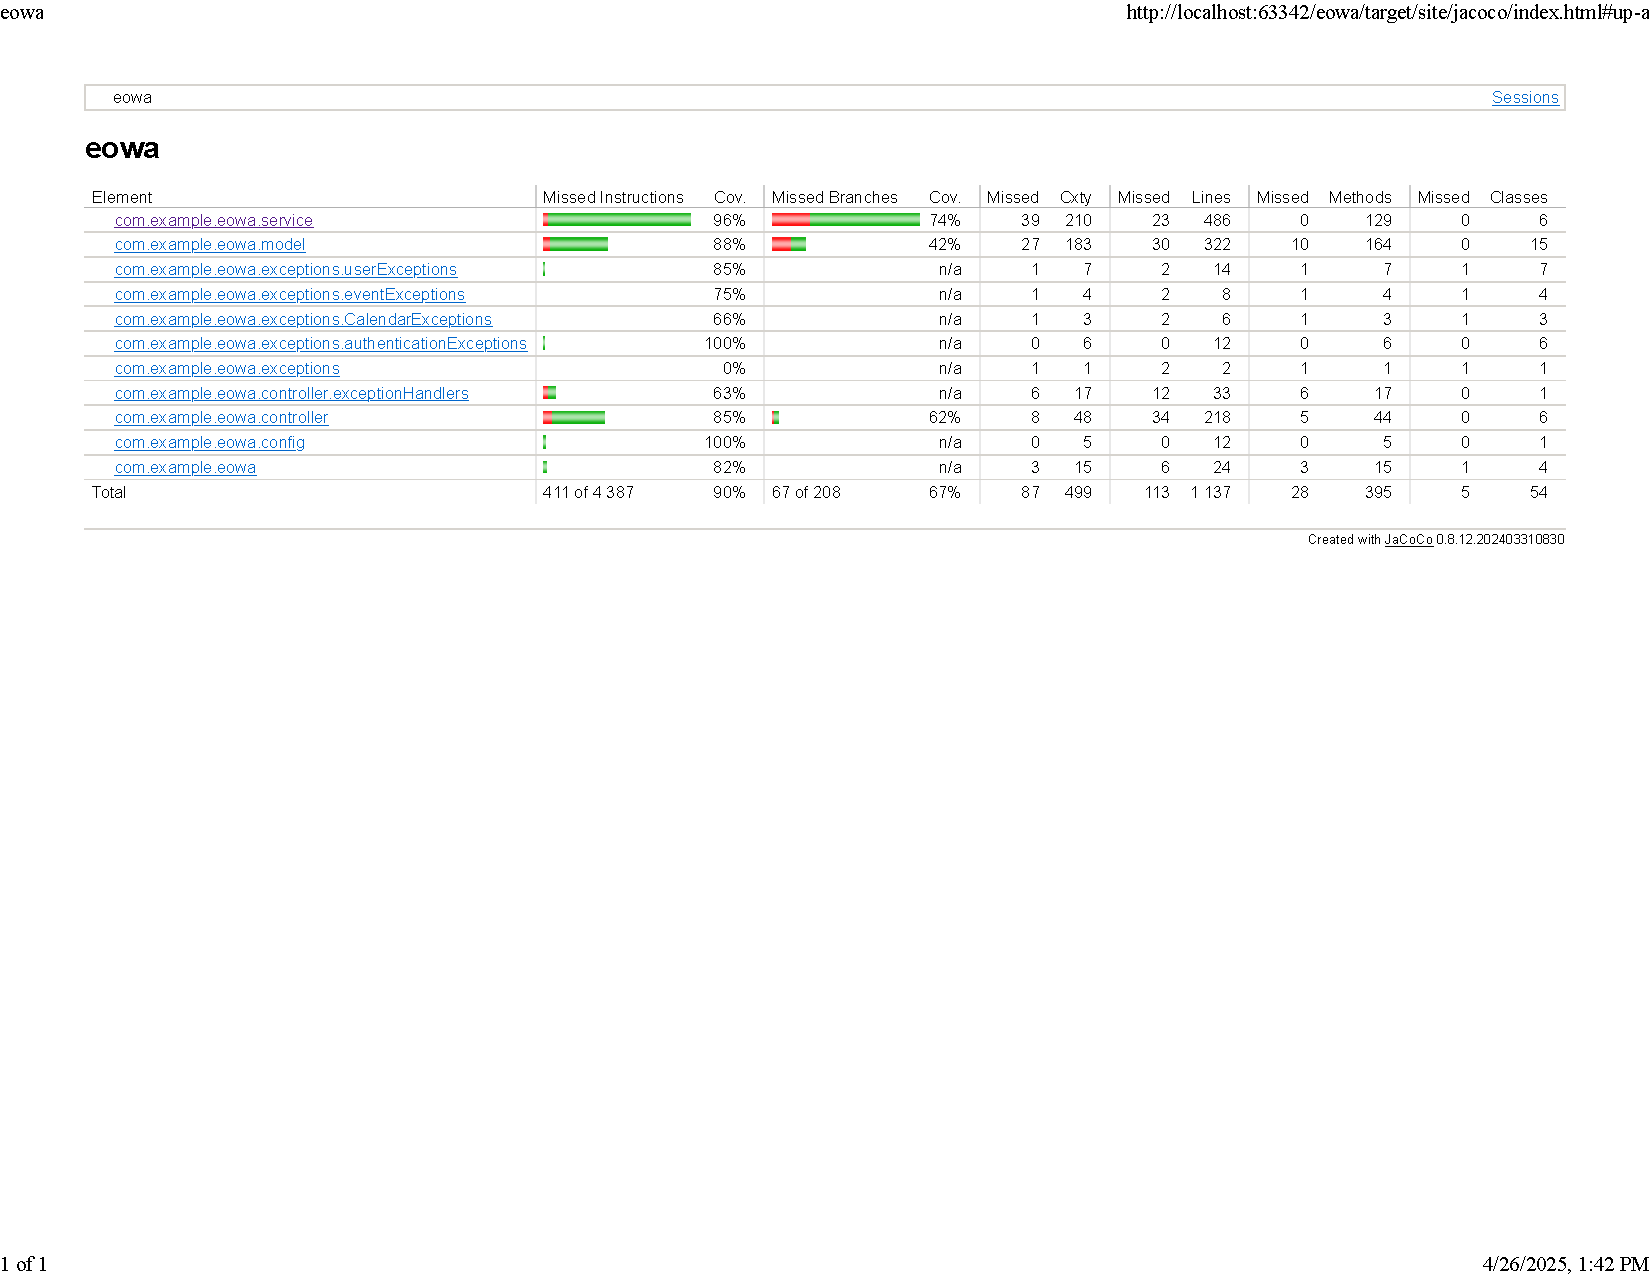
\includegraphics[width=170mm]{jacoco.pdf}

\end{center}

\subsection{Jacoco report a service rétegről}
\label{jacocoservice}
\begin{center}
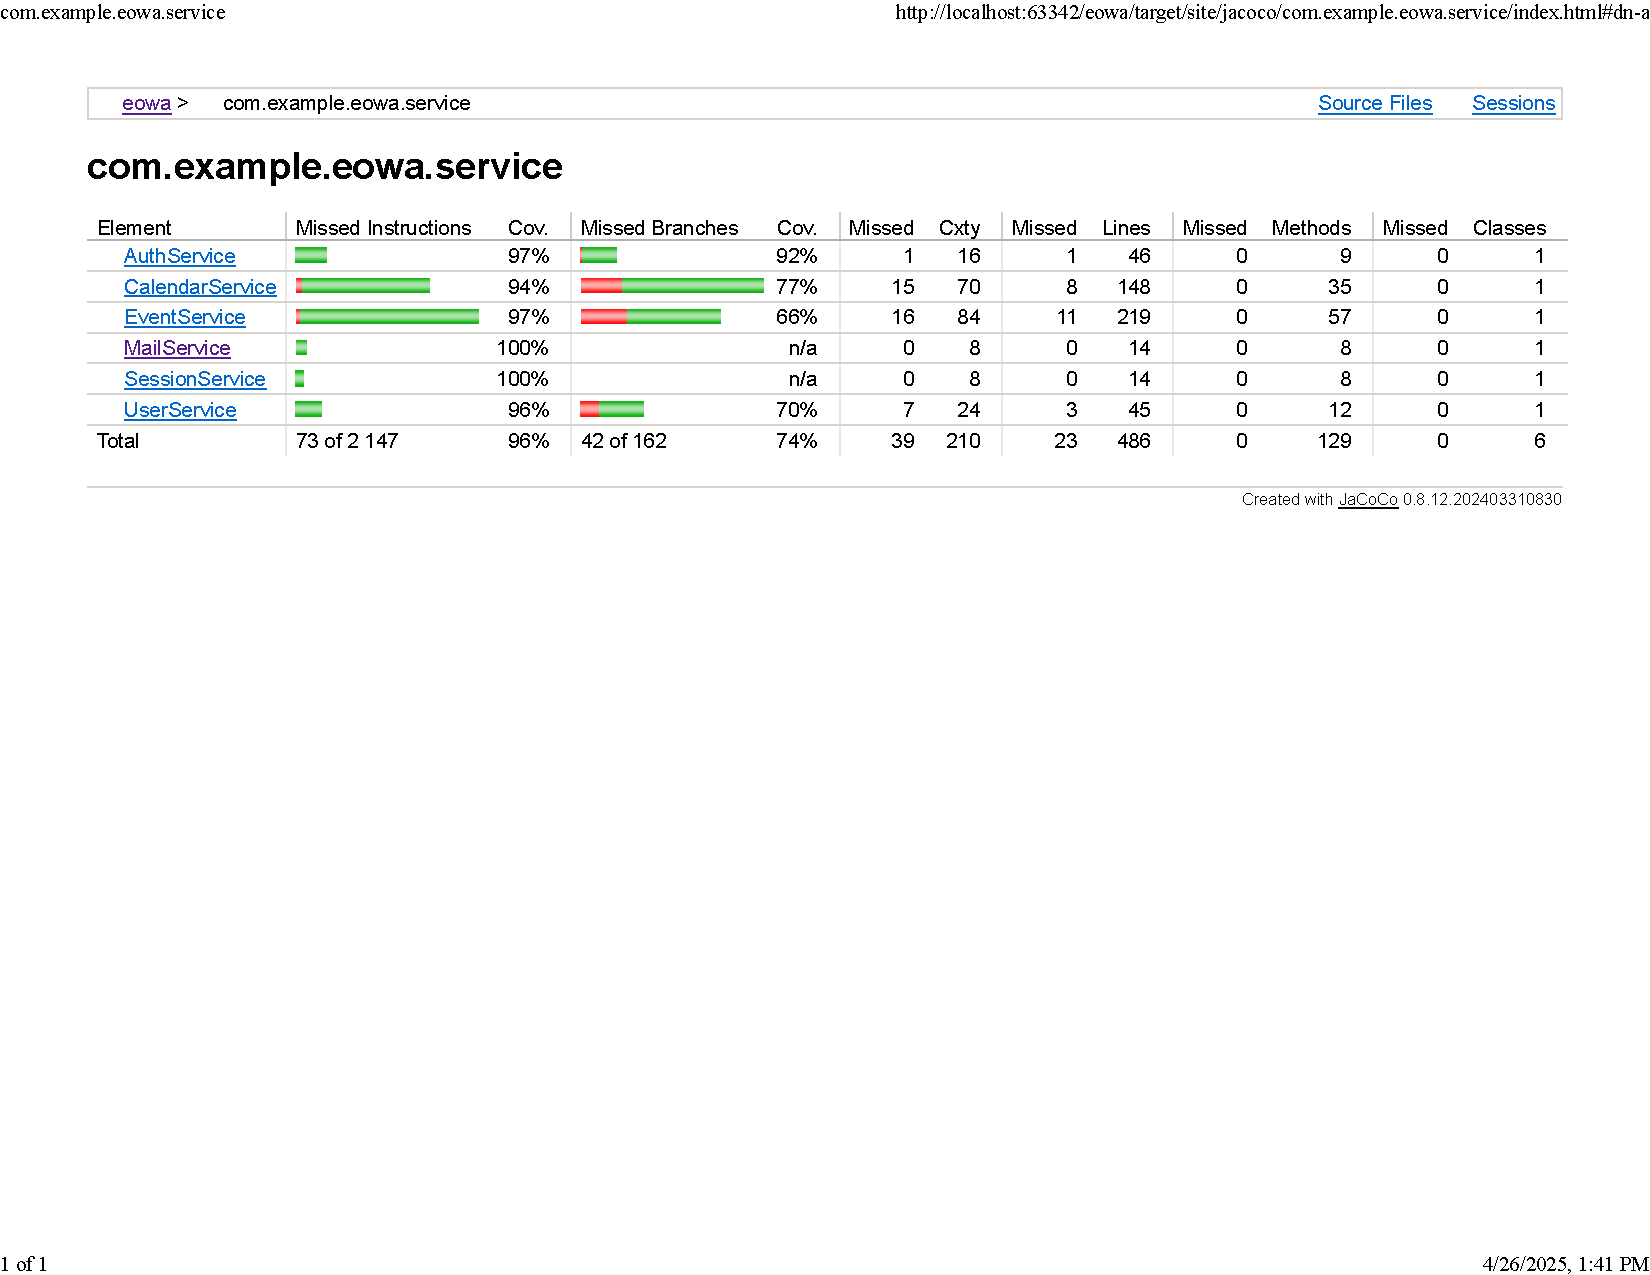
\includegraphics[width=170mm]{jacoco_service.pdf}

\end{center}


\vspace{2 cm}


\end{document}



